\documentclass[12pt]{article}
\usepackage[margin=1in]{geometry}
\usepackage{amsmath, amssymb, amsthm}
\usepackage{graphicx}
\usepackage{booktabs}
\usepackage{setspace}
\usepackage{xcolor}
\usepackage[colorlinks=true, linkcolor=blue!50!black, citecolor=blue!50!black, urlcolor=blue!50!black]{hyperref}
\usepackage{caption}
\usepackage{float}
\usepackage{natbib}
\bibliographystyle{apalike}

\newtheorem{proposition}{Proposition}

\onehalfspacing

\title{\textbf{The Long Shadow of Slavery: Plantation Intensity and Violent Crime in U.S.\ Counties, 1990--2016}\\[0.6em]
\large}
\author{Jacob Sharadin\thanks{Replication code and data construction scripts are available from the author.}}
\date{June 2026}

\begin{document}

\maketitle

\begin{abstract}
\noindent I study whether the intensity of slavery on the eve of the Civil War predicts violent crime in the same places a century and a half later. I link the full 1860 Census of Population and Agriculture to county-level FBI Uniform Crime Reports for 1990, 2000, 2010, and 2016, covering 1,071 counties in the fifteen slave states---an order of magnitude more counties than earlier drafts of this research design. Within states, and conditional on 1860 population, agricultural wealth, and immigrant share, a one-standard-deviation increase in a county's 1860 enslaved population share (22 percentage points) is associated with approximately 18\% higher violent crime in 2010; Poisson estimates for murder imply a similar magnitude. The association is far weaker for property crime, is robust to estimator and sample choices, and survives wild cluster bootstrap and Conley spatial-HAC inference, but declines monotonically across census years, from 1990 to 2016. An instrumental-variable exercise using FAO-GAEZ cotton suitability yields positive two-stage estimates consistent with---but too imprecise to sharpen---the OLS gradient. Contrary to a prominent hypothesized channel, I find no evidence that the persistence operates through historical land concentration: within states, the 1860 farm-size Gini coefficient is uncorrelated with slave intensity and does not predict modern crime, while the scale of slaveholding does. These results support cultural and institutional---rather than land-inequality---interpretations of slavery's criminogenic legacy, and caution against instrumental-variable designs that route slavery's effect exclusively through inequality.
\end{abstract}

\vspace{1em}

\newpage

\section{Introduction}

Economists have long argued that historical institutions cast long shadows over modern economic and social outcomes \citep{acemoglu2001, dell2010, nunn2008qje}. American slavery is perhaps the starkest case: it organized the economies of fifteen states around coerced labor, and its abolition was followed not by convergence but by a century of institutionalized exclusion, racial violence, and unequal development \citep{foner1988, sacerdote2005, oconnell2012}. A separate literature asks whether economic inequality causes crime, with theory predicting effects concentrated in violent rather than property crime and evidence that remains contested \citep{becker1968, kelly2000, fajnzylber2002, pazzona2024}. These literatures intersect in a natural question: do places that were more intensively organized around slavery in 1860 have more violent crime today, and if so, why?

This paper provides evidence on both parts of that question using, to my knowledge, the most complete county-level linkage of antebellum census data to modern crime records assembled for this design. I combine the National Historical Geographic Information System (NHGIS) tabulation of the complete 1860 Censuses of Population and Agriculture---which reports each county's enslaved population, farm values, the distribution of farms across acreage classes, and the distribution of slaveholdings across size classes---with the FBI Uniform Crime Reporting (UCR) county-level ``offenses known to police'' files for 1990, 2000, 2010, and 2016. A name-based crosswalk matches 98\% of 1860 slave-state counties to modern FIPS codes, yielding 1,071 counties observed in up to four modern census years.

The empirical design is deliberately a \emph{reduced-form persistence} design, not an instrumental-variables design. All identification comes from within-state comparisons: I regress modern crime on the 1860 enslaved share of county population, conditional on state fixed effects and 1860 county covariates (log population, farm value per capita, foreign-born share, and the share of farmland improved). Because treatment varies at the county level but unobserved law-enforcement and reporting practices vary at the state level, I cluster standard errors by state and confirm the main result with the wild cluster bootstrap of \citet{cgm2008}. Because murder is a rare count---41\% of sample counties recorded zero murders in 2010---I estimate count outcomes by Poisson pseudo-maximum-likelihood with population exposure \citep{santossilva2006} rather than logging rates.

Three findings emerge. First, the slavery--violence gradient is large and robust in the cross-section. Within states, a one-standard-deviation (22 percentage point) increase in the 1860 slave share predicts about 18\% more violent crime per capita in 2010 (wild cluster bootstrap $p = 0.001$); Poisson estimates for murder counts imply a comparable 15\%. The gradient for property crime is roughly one-third as large and only marginally significant---the same violent/property asymmetry found in the inequality--crime literature \citep{kelly2000} and in related work on slavery and crime in Colombia \citep{buonanno2019}.

Second, the gradient \emph{fades}. Estimated year by year, the coefficient falls monotonically from 1.10 (s.e.\ 0.21) in 1990 to 0.30 (s.e.\ 0.30) in 2016. The pooled panel estimate remains highly significant, but the trend suggests the criminogenic component of slavery's legacy has weakened over the past generation---a pattern consistent with \citet{abs2016}, who document that the attitudinal legacy of slavery, while persistent, attenuates with cohort replacement and migration.

Third, and most surprisingly, the leading hypothesized mechanism in the economics literature finds no support in these data. The Engerman--Sokoloff tradition holds that slavery generated persistent \emph{land} inequality, which in turn drives social dysfunction including crime \citep{engerman2002, nunn2008americas}. I construct each county's 1860 farm-size Gini coefficient from the seven acreage classes of the Census of Agriculture (Appendix~\ref{app:gini} shows the grouped statistic is a lower bound on the true Gini). Within states, slave intensity is essentially uncorrelated with the farm-size Gini ($\hat{\beta} = 0.015$, s.e.\ $0.022$): plantation counties did not have measurably more concentrated farm-size distributions than smallholding counties in the same state. The farm-size Gini, in turn, does not predict modern violent crime, and including it leaves the slave-share coefficient unchanged. What \emph{does} track slave intensity is the scale of slaveholding---slaves per slaveholder rises steeply with the slave share---indicating that the treatment is better understood as plantation economy intensity than as land concentration. These results favor cultural and institutional channels---the ``culture of violence'' and racialized enforcement legacies documented by historians \citep{tolnay1995, foner1988} and the political-attitude channel of \citet{abs2016}---and they imply a concrete methodological warning: instrumental-variable designs that use historical slavery as an instrument for inequality \citep[as in][]{buonanno2019} are unlikely to satisfy the exclusion restriction in the U.S. context, because slavery's effect on crime does not appear to route through the inequality variable being instrumented.

This paper is closest to \citet{gouda2025}, who document a positive association between 1860 slavery and county violent crime in census years 1970--2000 and explore inequality and political attitudes as mediators; Section~\ref{sec:gouda} provides a detailed comparison. My contribution relative to that work is fivefold: (i) I extend the outcome window to 2016 and document that the gradient declines sharply in the most recent data; (ii) I use offenses-known files (crimes reported) rather than arrest-based measures, separating the outcome from enforcement intensity; (iii) I treat rare counts with Poisson models rather than logged rates, which matters in a sample where two-fifths of counties record zero murders; (iv) I test the \emph{historical land concentration} mechanism directly with a farm-size Gini built from the same 1860 census as the treatment, rather than proxying inequality with modern income measures, and reject it; and (v) I subject the design to weak-instrument-robust IV inference and spatial-HAC standard errors, reporting transparently where the data can and cannot tighten identification. The paper also relates to work on slavery's legacy for education and income gaps \citep{sacerdote2005, bertocchi2014, oconnell2012} and to the broader persistence literature \citep{dell2010, nunn2008qje}.

The remainder of the paper proceeds as follows. Section~\ref{sec:background} sketches the historical setting and the candidate channels. Section~\ref{sec:data} describes the data and the construction of the analysis sample. Section~\ref{sec:strategy} lays out the empirical strategy and its identifying assumptions. Section~\ref{sec:results} presents the main results, Section~\ref{sec:mechanism} the mechanism analysis, and Section~\ref{sec:robust} robustness. Section~\ref{sec:conclusion} concludes.

\section{Historical background and conceptual framework}\label{sec:background}

\subsection{Slavery and the plantation South}

By 1860, just under four million people were enslaved in the United States, concentrated in a plantation belt running from the Chesapeake through the Black Belt of Alabama and Georgia to the Mississippi Valley and east Texas. Within slave states, the intensity of slavery varied enormously across counties: in my sample the enslaved share of county population ranges from zero in Appalachian and Ozark counties to 92\% in the richest cotton and rice districts, with a mean of 28\% (Table~\ref{tab:summary}). This within-state variation---mountain counties beside plantation counties under the same state law---is the variation exploited below.

Emancipation destroyed slavery as a labor system but not the local social order built on it. Reconstruction was followed by paramilitary violence, the convict-lease system, disenfranchisement, and Jim Crow \citep{foner1988}. Lynching was concentrated precisely in former plantation counties \citep{tolnay1995}. \citet{abs2016} show that whites in high-slavery counties today express systematically different racial and political attitudes than whites in nearby low-slavery counties, and attribute the divergence to the incentives of the planter class after emancipation. \citet{sacerdote2005} and \citet{bertocchi2014} document long-lived effects on Black human capital accumulation.

\subsection{Channels from slavery to modern crime}

Four channels could generate a slavery--crime gradient a century and a half later.

\emph{Land and wealth inequality.} In the Engerman--Sokoloff hypothesis, factor endowments suited to plantation agriculture generated concentrated landownership and institutions protecting elite interests, retarding broad-based development \citep{engerman2002, nunn2008americas}. If economic inequality causes violent crime \citep{kelly2000, fajnzylber2002}, persistent land concentration is a candidate mechanism. This channel is testable here: the 1860 Census of Agriculture reports the distribution of farms across acreage classes, from which a county-level farm-size Gini can be constructed.

\emph{Culture of violence and weak legitimate enforcement.} Slavery was maintained by private violence, and post-emancipation racial control operated through extralegal violence tolerated or assisted by local authorities \citep{tolnay1995}. A durable equilibrium of low trust in legal institutions and high private violence would raise violent crime specifically, with little effect on property crime---matching the asymmetry found below.

\emph{Poverty and underdevelopment.} Former plantation counties remain poorer, with worse schooling and health \citep{oconnell2012, bertocchi2014}. Economic deprivation raises both violent and property crime in standard models \citep{becker1968}, so this channel predicts effects on both margins.

\emph{Demographic composition and discrimination.} High-slavery counties have larger Black populations today, who face concentrated disadvantage and discriminatory enforcement. The reduced form estimated below deliberately does \emph{not} condition on modern racial composition or income, which are themselves outcomes of the treatment; the estimand is the \emph{total} long-run association running through all downstream channels, in the spirit of \citet{abs2016}. Section~\ref{sec:mechanism} then asks which intermediate variables the data can rule in or out.

\section{Data}\label{sec:data}

\subsection{1860 census data}

The treatment and historical covariates come from the NHGIS county tabulations of the 1860 Censuses of Population and Agriculture \citep{nhgis}. For each of the 1,112 counties of the fifteen slave states (Alabama, Arkansas, Delaware, Florida, Georgia, Kentucky, Louisiana, Maryland, Mississippi, Missouri, North Carolina, South Carolina, Tennessee, Texas, and Virginia, which then included West Virginia), I observe total population by status (white, free colored, enslaved), nativity, the cash value of farms, improved and unimproved farm acreage, the number of farms in seven acreage classes (3--9, 10--19, 20--49, 50--99, 100--499, 500--999, and 1{,}000+ acres), and the number of slaveholders in twenty-one holding-size classes.

The treatment variable is the \emph{enslaved share of county population},
$SlaveShare_i = \text{Slaves}_i / \text{Population}_i$,
a bounded intensity measure comparable across counties of different sizes. (Earlier drafts of this project used the log \emph{count} of enslaved people, which conflates slavery intensity with county scale.) Historical controls are log county population, log farm value per capita, the foreign-born population share, and the improved share of farm acreage, all measured in 1860 and therefore pre-determined with respect to modern outcomes.

From the farm acreage classes I construct a county farm-size Gini coefficient by assigning each farm its class midpoint (with the open top class set to 1{,}500 acres) and computing the Gini over the resulting grouped distribution. Proposition~\ref{prop:gini} in Appendix~\ref{app:gini} establishes that the grouped statistic bounds the true farm-size Gini from below, so cross-county comparisons are conservative with respect to within-class dispersion. From the slaveholding classes I construct average slaves per slaveholder, a measure of plantation scale.

\subsection{Modern crime data}

Modern outcomes come from the ICPSR county-level UCR files for 1990, 2000, 2010, and 2016 \citep{ucr2010}---specifically the ``Crimes Reported'' (offenses known to police) parts, not the arrest files. Offenses known are the standard outcome in the crime literature because arrests confound criminal activity with enforcement effort. Each file reports murders, rapes, robberies, aggravated assaults, burglaries, larcenies, and motor-vehicle thefts, together with the population covered by reporting agencies; agencies reporting 6--11 months are weighted to annual equivalents by ICPSR. I define violent crime as murder + rape + robbery + aggravated assault and property crime as burglary + larceny + motor-vehicle theft, expressed per 100,000 covered population. Counties with zero covered population in a year are excluded; robustness checks restrict to counties with high coverage indices and weight by covered population.

Two features of the outcome data shape the econometrics. First, violent crime rates are strictly positive in 99\% of county-years, so logs are usable; but \emph{murder} is zero in 41\% of counties in 2010. Logging murder rates would either discard those counties or require arbitrary adjustments to zeros---a problem in earlier drafts of this project---so murder is modeled as a count by Poisson pseudo-maximum likelihood with the log of covered population as exposure \citep{santossilva2006}. Second, UCR county coverage deteriorates in later years and varies across states, motivating the coverage-restricted robustness checks and the state-clustered inference described below.

\subsection{Linking 1860 counties to modern counties}

I match 1860 counties to modern FIPS codes by normalized county name within state, allowing 1860 Virginia counties to match modern West Virginia counties. The crosswalk matches 1,090 of 1,112 counties (98.0\%); unmatched cases are mostly renamed or dissolved counties. Where multiple 1860 counties map to one modern county, the first match is retained. The 2010 analysis sample contains 1,071 counties with positive covered population---compared with 126 counties in an earlier draft of this design, which had also inadvertently pooled county records across states because ICPSR county codes repeat within every state. All results below use the corrected, near-universe sample. County boundaries changed between 1860 and the modern period, particularly in Texas and Florida; name matching keeps the stable majority and measurement error from boundary changes should attenuate, not inflate, the estimates.

\begin{table}[H]
\centering
\caption{Summary statistics, 2010 analysis sample}
\label{tab:summary}
\begin{tabular}{lcccccc}
\toprule
 & Mean & SD & Min & Median & Max & $N$ \\
\midrule
Slave share of population, 1860 & 0.283 & 0.220 & 0.000 & 0.242 & 0.923 & 1,071 \\
Land Gini (farm acreage), 1860 & 0.491 & 0.074 & 0.158 & 0.493 & 0.833 & 1,050 \\
County population, 1860 & 11,119 & 12,546 & 26 & 8,917 & 212,418 & 1,071 \\
Cash value of farms (\$), 1860 & 2,367,788 & 2,530,216 & 500 & 1,536,178 & 22,491,196 & 1,056 \\
Violent crime rate per 100k, 2010 & 305 & 238 & 0 & 240 & 2,267 & 1,071 \\
Murder rate per 100k, 2010 & 4.005 & 5.796 & 0.000 & 2.443 & 53.430 & 1,071 \\
Property crime rate per 100k, 2010 & 2,402 & 1,337 & 0 & 2,272 & 8,853 & 1,071 \\
\bottomrule
\end{tabular}
\par\smallskip
\footnotesize\textit{Notes:} Counties of the fifteen 1860 slave states matched to modern FIPS codes with positive UCR covered population in 2010. Crime rates are offenses known to police per 100,000 covered population. The land Gini is computed from grouped farm-acreage classes (Appendix~\ref{app:gini}).
\end{table}

Table~\ref{tab:summary} reports summary statistics and Figure~\ref{fig:hist} the distribution of the treatment. The 2010 violent crime rate averages 305 per 100,000 with wide dispersion; the murder rate averages 4.0. The farm-size Gini averages 0.49 with substantial variation (0.16--0.83).

\section{Empirical strategy}\label{sec:strategy}

\subsection{Specification}

The baseline specification for continuous outcomes is
\begin{equation}\label{eq:ols}
\log y_{is} = \beta \, SlaveShare_{is} + X_{is}'\gamma + \alpha_s + \varepsilon_{is},
\end{equation}
where $y_{is}$ is the violent (or property) crime rate of county $i$ in state $s$ in a given modern year, $X_{is}$ contains the 1860 covariates, and $\alpha_s$ are state fixed effects. For murder, the count analogue is estimated by Poisson pseudo-maximum likelihood:
\begin{equation}\label{eq:ppml}
E[\,\text{Murders}_{is} \mid \cdot\,] = \exp\!\big(\log \text{Pop}^{cov}_{is} + \beta \, SlaveShare_{is} + X_{is}'\gamma + \alpha_s\big),
\end{equation}
with the covered population entering as exposure with a unit coefficient. In both cases $\beta$ is a semi-elasticity: $100 \cdot [\exp(\beta \sigma) - 1]$ is the percentage change in crime associated with a $\sigma$-unit increase in the slave share.

For the panel, I pool the four census years with year fixed effects and cluster by county; I also report each year separately.

\subsection{Identification and inference}

Equation~\eqref{eq:ols} is a selection-on-observables design within states. The identifying assumption is that, conditional on state fixed effects and the 1860 covariates, the determinants of where slavery was intensive within a state---chiefly soils, climate, and river access suited to plantation crops---do not affect crime in 2010 through channels other than the legacy of slavery itself. This assumption is not innocuous: cotton-suitable geography could matter for modern outcomes through agricultural decline, for example. Three considerations support the design. First, all comparisons are within-state, absorbing state law, policing institutions, and UCR reporting conventions. Second, the 1860 controls capture the level of development (population, farm value per capita), immigration, and land improvement, so $\beta$ is not driven by plantation counties simply being richer or more settled in 1860. Third, the coefficient is remarkably stable as controls are added (Section~\ref{sec:results}), and the leave-one-state-out range is tight, suggesting the estimate is not an artifact of a particular confounder or region. I interpret $\beta$ as the total long-run association of plantation intensity with modern violence---a persistence parameter in the sense of \citet{abs2016}---rather than the causal effect of any single intermediate variable.

I do \emph{not} use slavery as an instrument for inequality, as in \citet{buonanno2019} and in an earlier draft of this project. The exclusion restriction required---that slavery affects crime \emph{only} through measured inequality---is directly contradicted by the mechanism evidence in Section~\ref{sec:mechanism}, where slavery's association with crime survives conditioning on historical land inequality entirely.

Treatment varies at the county level, but enforcement and reporting environments vary at the state level, so I cluster standard errors by state. With only fifteen clusters, cluster-robust standard errors can over-reject; for the main specification I therefore also report the wild cluster bootstrap $p$-value with Rademacher weights and the null imposed \citep{cgm2008}, with 999 replications. Because both slavery and crime are spatially autocorrelated within states, Section~\ref{sec:probe} additionally reports \citet{conley1999} spatial-HAC standard errors based on county centroids, and probes the selection-on-observables assumption directly with a cotton-suitability instrument.

\section{Main results}\label{sec:results}

\subsection{Cross-section, 2010}

\begin{table}[H]
\centering
\caption{Slavery in 1860 and crime in 2010: OLS}
\label{tab:ols}
\begin{tabular}{lccc}
\toprule
 & (1) & (2) & (3) \\
\midrule
\multicolumn{4}{l}{\textbf{Panel A. Dependent variable: log violent crime rate, 2010}} \\
Slave share, 1860 & 1.017*** & 0.713** & 0.769*** \\
 & (0.350) & (0.306) & (0.264) \\
\addlinespace
\multicolumn{4}{l}{\textbf{Panel B. Dependent variable: log property crime rate, 2010}} \\
Slave share, 1860 & 0.531*** & 0.351** & 0.265* \\
 & (0.198) & (0.166) & (0.144) \\
\midrule
State fixed effects & & Y & Y \\
1860 county controls & & & Y \\
Observations (Panel A) & 1,064 & 1,064 & 1,050 \\
Observations (Panel B) & 1,070 & 1,070 & 1,055 \\
\bottomrule
\end{tabular}
\par\smallskip
\footnotesize\textit{Notes:} OLS estimates of equation~\eqref{eq:ols}. Standard errors clustered by state (15 clusters) in parentheses. 1860 county controls: log population, log farm value per capita, foreign-born share, improved share of farm acreage. Wild cluster bootstrap $p$-value for the slave-share coefficient in column (3), Panel A: $p = 0.001$. * $p<0.10$, ** $p<0.05$, *** $p<0.01$.
\end{table}

Table~\ref{tab:ols} reports OLS estimates for 2010. The bivariate association (column 1) of 1.02 falls modestly to 0.71 with state fixed effects (column 2) and is 0.77 (s.e.\ 0.26) with full 1860 controls (column 3); the wild cluster bootstrap $p$-value is 0.001. The stability of the coefficient across columns---it \emph{rises} slightly when controls are added to the within-state specification---suggests that selection on the included observables is not driving the association \citep[in the spirit of][]{altonji2005}. Quantitatively, a one-standard-deviation increase in the 1860 slave share (22 percentage points) is associated with $100\cdot[\exp(0.769 \times 0.220)-1] \approx 18\%$ higher violent crime per capita. Moving from a county with no slavery to a median plantation county (slave share $\approx 0.45$) implies roughly 41\% higher violent crime.

Panel B shows the same specifications for property crime. The full-specification coefficient, 0.26 (s.e.\ 0.14), is one-third the violent-crime coefficient and only marginally significant. The violent/property asymmetry echoes \citet{kelly2000} on inequality and \citet{buonanno2019} on slavery in Colombia, and is consistent with channels that operate through interpersonal violence norms and enforcement legitimacy rather than through material deprivation alone, which should raise property crime as well \citep{becker1968}.

Figure~\ref{fig:binscatter} shows the within-state relationship nonparametrically: vigintile means of residualized log violent crime against residualized slave share are close to linear across the support.

\begin{figure}[H]
\centering
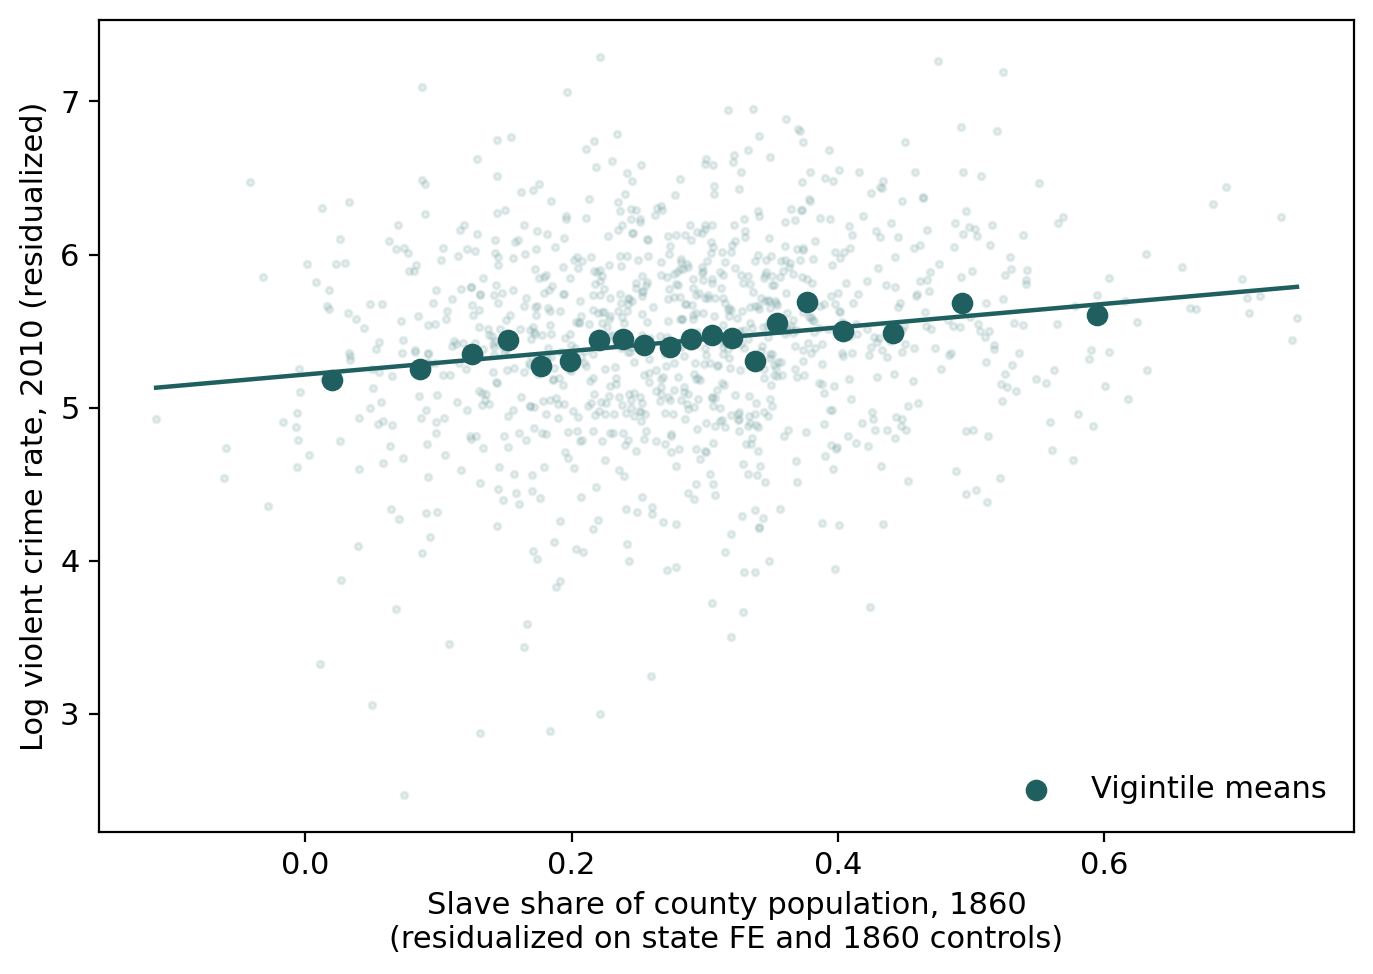
\includegraphics[width=0.78\textwidth]{output/figures/f1_binscatter.png}
\caption{Slave share in 1860 and log violent crime in 2010, within states. Both variables are residualized on state fixed effects and 1860 controls; points are county observations, dark dots are vigintile means, and the line is the OLS fit. $N = 1{,}050$.}
\label{fig:binscatter}
\end{figure}

\begin{table}[H]
\centering
\caption{Slavery in 1860 and murder in 2010: Poisson pseudo-maximum likelihood}
\label{tab:ppml}
\begin{tabular}{lccc}
\toprule
 & (1) & (2) & (3) \\
\midrule
\multicolumn{4}{l}{\textbf{Dependent variable: murder count, 2010 (exposure: covered population)}} \\
Slave share, 1860 & 0.379 & -0.081 & 0.634* \\
 & (0.257) & (0.511) & (0.349) \\
\midrule
State fixed effects & & Y & Y \\
1860 county controls & & & Y \\
Observations & 1,071 & 1,071 & 1,056 \\
\bottomrule
\end{tabular}
\par\smallskip
\footnotesize\textit{Notes:} PPML estimates of equation~\eqref{eq:ppml}; log covered population enters as exposure. Standard errors clustered by state in parentheses. 41\% of counties record zero murders in 2010 and are retained by the count specification. * $p<0.10$, ** $p<0.05$, *** $p<0.01$.
\end{table}

Table~\ref{tab:ppml} turns to murder, the best-measured violent crime. With state fixed effects and controls, the PPML coefficient is 0.63 (s.e.\ 0.35, $p = 0.07$), implying 15\% more murders per standard deviation of slave share. The murder estimates are noisier than the violent-index estimates, as expected for a rare count averaging four per 100,000---and the specification with state fixed effects but no controls is unstable---but the full specification is economically consistent with Panel A of Table~\ref{tab:ols}.

\subsection{Four decades of crime data}

\begin{table}[H]
\centering
\caption{The slavery--violence gradient across census years}
\label{tab:panel}
\begin{tabular}{lccc}
\toprule
UCR year & Coefficient & SE & $N$ \\
\midrule
1990 & 1.104*** & (0.210) & 989 \\
2000 & 0.735** & (0.329) & 924 \\
2010 & 0.769*** & (0.264) & 1,050 \\
2016 & 0.299 & (0.302) & 1,035 \\
\midrule
Pooled (year FE, county-clustered) & 0.717*** & (0.111) & 3,998 \\
\bottomrule
\end{tabular}
\par\smallskip
\footnotesize\textit{Notes:} Each row in the top panel is a separate estimate of equation~\eqref{eq:ols} (column 3 specification of Table~\ref{tab:ols}) for the indicated year, with state-clustered standard errors. The pooled specification adds year fixed effects and clusters by county (1,071 counties).
\end{table}

Table~\ref{tab:panel} and Figure~\ref{fig:byyear} estimate the gradient separately by UCR year. The pooled estimate is 0.72 (s.e.\ 0.11). But the year-by-year pattern is striking: 1.10 in 1990, 0.74 in 2000, 0.77 in 2010, and 0.30 (insignificant) in 2016. Two readings are possible. The substantive reading is convergence: the criminogenic component of the plantation legacy is fading, consistent with cohort replacement, migration, and the broader post-1990 crime decline compressing regional differences. The measurement reading is that UCR county coverage deteriorates in the 2010s as agencies transition to NIBRS reporting, differentially adding noise. The coverage-restricted robustness checks below somewhat favor the substantive reading---the 2010 estimate is essentially unchanged when low-coverage counties are dropped---but the 2016 decline should be interpreted with both candidates in mind, and the fading gradient is itself a finding worth further study: persistence is not permanence.

\begin{figure}[H]
\centering
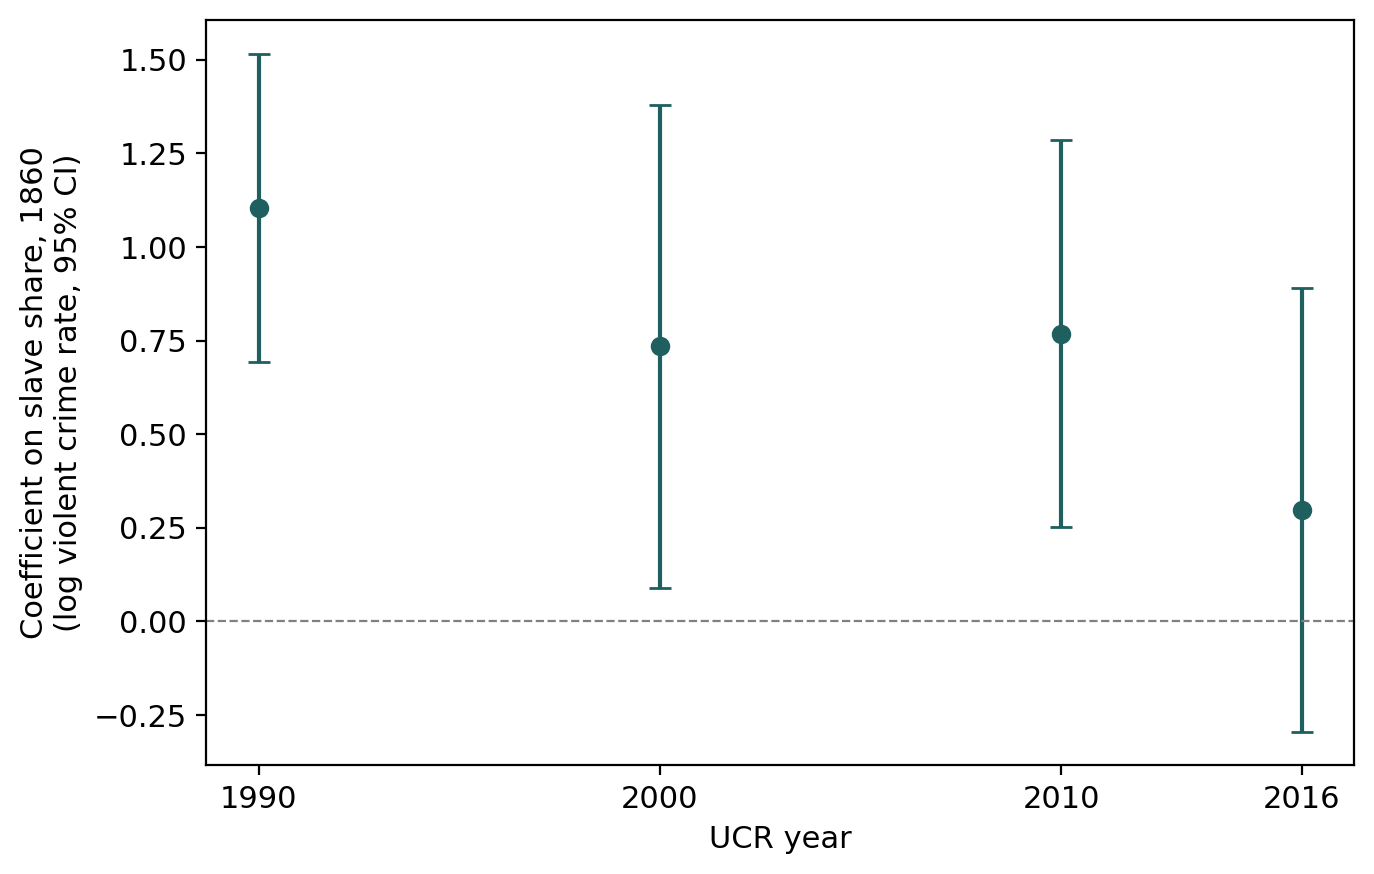
\includegraphics[width=0.7\textwidth]{output/figures/f2_byyear.png}
\caption{Coefficient on 1860 slave share by UCR year. Each point is the column-3 specification of Table~\ref{tab:ols} estimated for that year; bars are 95\% confidence intervals with state-clustered standard errors.}
\label{fig:byyear}
\end{figure}

\section{Mechanisms: land inequality versus plantation scale}\label{sec:mechanism}

The Engerman--Sokoloff channel predicts that slavery's legacy operates through concentrated landholding. The 1860 census permits a direct test that does not require modern mediators: if the channel is active, (i) slave intensity should predict the farm-size Gini in 1860, and (ii) the 1860 farm-size Gini should predict modern crime.

\begin{table}[H]
\centering
\caption{Mechanism evidence: land concentration and plantation scale, 1860}
\label{tab:mechanism}
\begin{tabular}{lcccc}
\toprule
 & (1) & (2) & (3) & (4) \\
Dep.\ var. & Land Gini & Slaves/holder & \multicolumn{2}{c}{Log violent crime, 2010} \\
\midrule
Slave share, 1860 & 0.015 & 21.535*** &  & 0.735*** \\
 & (0.022) & (1.607) &  & (0.258) \\
Land Gini, 1860 &  &  & -0.061 & -0.122 \\
 &  &  & (0.383) & (0.384) \\
\midrule
State FE \& 1860 controls & Y & Y & Y & Y \\
Observations & 1,048 & 1,043 & 1,042 & 1,042 \\
\bottomrule
\end{tabular}
\par\smallskip
\footnotesize\textit{Notes:} All columns include state fixed effects and 1860 controls; state-clustered standard errors in parentheses. Columns (1)--(2): 1860 outcomes regressed on 1860 slave share. Columns (3)--(4): 2010 log violent crime regressed on the 1860 land Gini, without and with the slave share. * $p<0.10$, ** $p<0.05$, *** $p<0.01$.
\end{table}

Table~\ref{tab:mechanism} rejects both premises. Column (1): within states, the slave share is essentially unrelated to the farm-size Gini (coefficient 0.015, s.e.\ 0.022)---plantation counties did not have more unequal farm-size distributions than smallholding counties in the same state, a pattern visible nonparametrically in Figure~\ref{fig:gini}. Column (2) shows what \emph{did} differ: average slaves per slaveholder rises by 21.5 (s.e.\ 1.6) moving from a zero-slavery to an all-slave county---plantation scale, not farm-size concentration, is the footprint of slavery in the agricultural census. Column (3): the 1860 land Gini does not predict 2010 violent crime ($-0.06$, s.e.\ 0.38). Column (4): including the land Gini leaves the slave-share coefficient essentially unchanged (0.74 versus 0.77 in the baseline).

Three caveats qualify the null. The farm-size Gini is computed over \emph{farms}, not landowners, and excludes the landless---enslaved people above all---so it measures concentration within the farming sector rather than wealth inequality in the full population; a Gini over all households including the enslaved (who owned nothing) would be mechanically increasing in the slave share. It is based on acreage, not value, and grouped into classes (though Proposition~\ref{prop:gini} shows grouping biases the level down, not the cross-county ordering, under within-class homogeneity). And measured in 1860 it cannot capture post-bellum land dynamics such as plantation subdivision into tenancies. With those caveats, the data are nonetheless inconsistent with the simplest land-concentration story: whatever transmits the plantation legacy into modern violence, it is not well proxied by the antebellum farm-size distribution. This is consistent with \citet{gouda2025}, who find that \emph{modern} income inequality and political attitudes mediate part of the slavery--crime association, and with \citet{abs2016}, who locate the legacy in persistent local culture and institutions rather than factor distributions. It is, however, bad news for designs that instrument inequality with slavery \citep{buonanno2019}: in these data, slavery moves crime without moving the historical inequality measure at all, a textbook exclusion-restriction failure.

\begin{figure}[H]
\centering
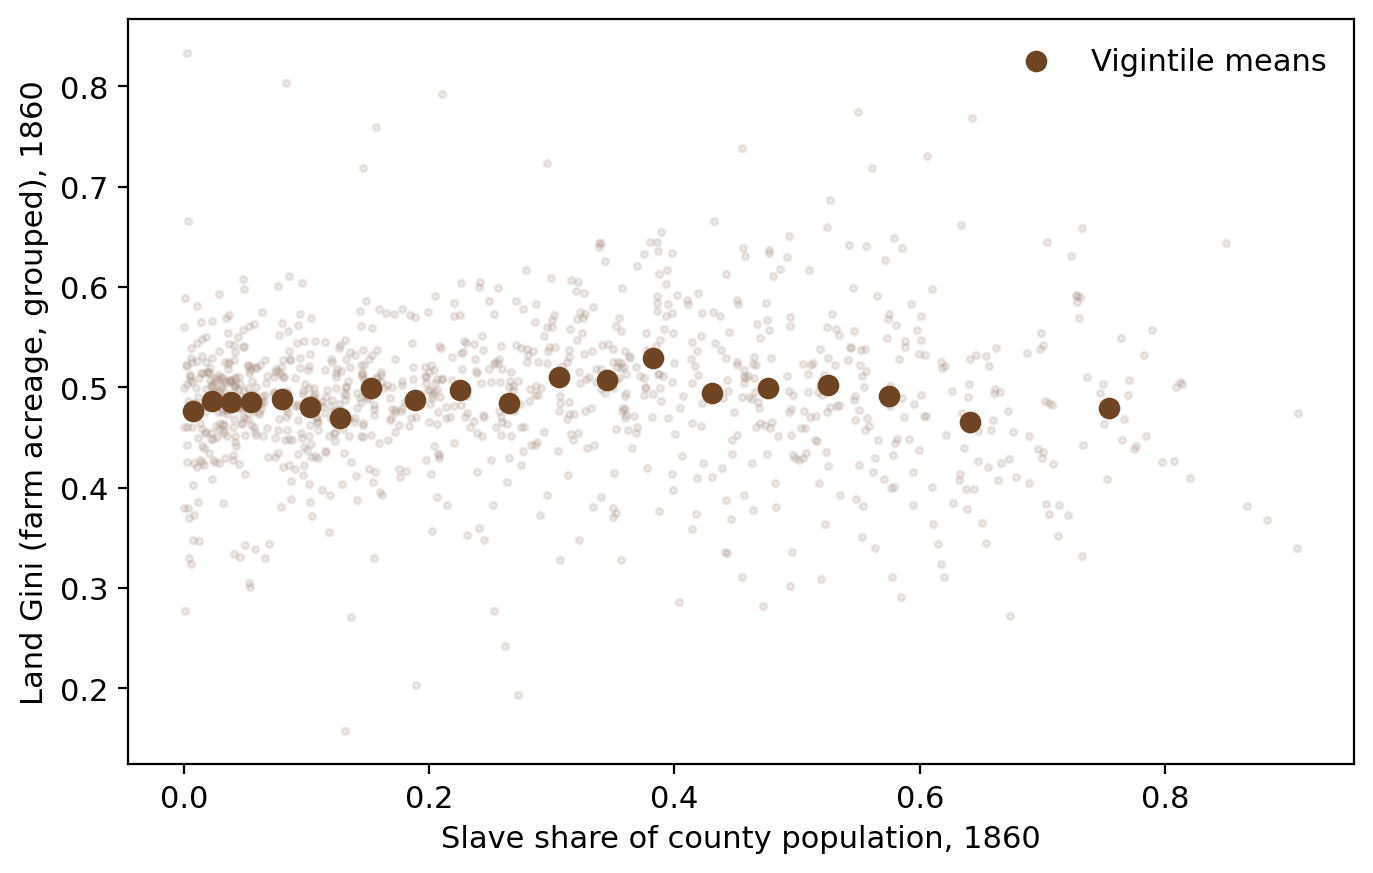
\includegraphics[width=0.72\textwidth]{output/figures/f3_gini.png}
\caption{Slave share and the farm-size Gini across counties, 1860. Dark dots are vigintile means. The raw correlation is weakly positive across states but disappears within states (Table~\ref{tab:mechanism}, column 1).}
\label{fig:gini}
\end{figure}

\section{Robustness}\label{sec:robust}

\begin{table}[H]
\centering
\caption{Robustness of the main estimate}
\label{tab:robust}
\begin{tabular}{lccc}
\toprule
Specification & Coefficient & SE & $N$ \\
\midrule
Baseline (col. 3, Table 2) & 0.769*** & (0.264) & 1,050 \\
UCR coverage index $\geq$ 75 & 0.753*** & (0.258) & 1,030 \\
Weighted by covered population & 0.528*** & (0.170) & 1,050 \\
asinh(violent crime rate) & 0.841*** & (0.271) & 1,056 \\
Excluding Virginia & 1.083*** & (0.204) & 915 \\
Violent rate winsorized at 1/99 pct. & 0.781*** & (0.264) & 1,056 \\
\bottomrule
\end{tabular}
\par\smallskip
\footnotesize\textit{Notes:} Variations on column (3), Panel A of Table~\ref{tab:ols}. State-clustered standard errors. * $p<0.10$, ** $p<0.05$, *** $p<0.01$.
\end{table}

Table~\ref{tab:robust} probes the 2010 violent-crime estimate. Restricting to counties with UCR coverage indices of at least 75 leaves the coefficient unchanged (0.75), easing concerns that differential reporting drives the result. Weighting by covered population yields 0.53---smaller, indicating the gradient is steeper among less populous counties, but strongly significant. Using the inverse hyperbolic sine instead of logs (0.84), winsorizing the outcome at the 1st and 99th percentiles (0.78), and excluding Virginia with its independent-city geography (1.08) all preserve the finding. Across leave-one-state-out samples the coefficient ranges from 0.67 to 1.08, always significant at the 1\% level. The estimate is not driven by any single state, by outliers, by functional form, or by low-coverage counties.

\section{Probing identification}\label{sec:probe}

This section subjects the design to three further tests: a geographic instrument for slave intensity, spatial-dependence-robust inference, and a structured comparison with the closest prior study. Throughout, I merge in county-level cotton suitability from the FAO-GAEZ-based measure constructed by \citet{absdata} and county centroids from the Census gazetteer. The merge also provides an external check on the dataset construction: the correlation between my NHGIS-built slave share and the \citet{abs2016} county slave proportion is 0.998.

\subsection{A cotton-suitability instrument}\label{sec:iv}

Where slavery took hold within a state was determined in large part by agronomy: cotton (with sugar and rice) made large-scale coerced labor profitable. Following \citet{abs2016}, I use county cotton suitability---a function of soil and climate, fixed before settlement---as an instrument for the 1860 slave share. The exclusion restriction is that, within states and conditional on the controls, cotton-growing geography affects modern violent crime only through the plantation system it induced. This is disputable (suitability also shaped post-bellum agriculture and exposure to the Boll Weevil and the Great Migration), so I read the exercise as a consistency check on the OLS gradient rather than as a superior estimate.

\begin{table}[H]
\centering
\caption{Cotton suitability as an instrument for slave intensity}
\label{tab:iv}
\begin{tabular}{lccc}
\toprule
 & (1) & (2) & (3) \\
\midrule
\multicolumn{4}{l}{\textbf{Panel A. First stage. Dep.\ var.: slave share, 1860}} \\
Cotton suitability & 0.452*** & 0.268** & \\
 & (0.096) & (0.112) & \\
First-stage $F$ & 22.2 & 5.7 & \\
\addlinespace
\multicolumn{4}{l}{\textbf{Panel B. Dep.\ var.: log violent crime rate, 2010}} \\
Slave share, 1860 (2SLS) & 0.367 & 0.844 & \\
 & (0.606) & (1.002) & \\
Cotton suitability (reduced form) & & & 0.166 \\
 & & & (0.286) \\
\addlinespace
\multicolumn{4}{l}{\textbf{Panel C. Dep.\ var.: log property crime rate, 2010 (2SLS)}} \\
Slave share, 1860 & 0.203 & & \\
 & (0.557) & & \\
\midrule
State FE \& log 1860 population & Y & Y & Y \\
Full 1860 controls & & Y & \\
Observations & 1,021 & 1,007 & 1,021 \\
\bottomrule
\end{tabular}
\par\smallskip
\footnotesize\textit{Notes:} Just-identified 2SLS with state-clustered standard errors in parentheses; cotton suitability from \citet{absdata}. Column (1) conditions on state fixed effects and log 1860 population; column (2) adds the full 1860 controls (farm value per capita, foreign-born share, improved acreage share); column (3) reports the reduced form of column (1). The weak-instrument-robust \citet{andersonrubin1949} 95\% confidence set for the column-(2) coefficient is $[-5.4,\, 2.8]$. * $p<0.10$, ** $p<0.05$, *** $p<0.01$.
\end{table}

Table~\ref{tab:iv} reports the results, which are informative in both directions. With state fixed effects and log population, the first stage is strong: a one-unit increase in cotton suitability raises the slave share by 0.45 (s.e.\ 0.10), with a first-stage $F$ of 22, comfortably above conventional thresholds \citep{staigerstock1997}. The corresponding 2SLS estimate is 0.37 (s.e.\ 0.61): positive, within one standard error of the OLS estimate of 0.77, but too imprecise to distinguish from zero or from twice the OLS magnitude. Adding the full 1860 controls (column 2) raises the point estimate to 0.84---almost exactly the OLS coefficient---but the first-stage $F$ falls to 5.7, because farm values and improved acreage are themselves products of suitability; the weak-instrument-robust Anderson--Rubin 95\% confidence set, $[-5.4, 2.8]$, brackets the OLS estimate without excluding zero. The property-crime 2SLS (Panel C) is small and insignificant, mirroring the OLS asymmetry.

The honest summary is that the instrument \emph{cannot adjudicate}: every IV point estimate is positive and consistent with the OLS gradient, and none is precise. The deeper lesson is about the design space. Cotton suitability earns its strength from variation that is partly absorbed by development controls, and its exclusion logic weakens exactly when those controls are removed---a tension that should temper confidence in suitability-instrumented designs generally, including applications that instrument \emph{inequality} with slavery-related variables \citep{buonanno2019}.

\subsection{Spatial dependence}\label{sec:conley}

Plantation agriculture followed soil belts that cross county lines, so residuals are likely spatially correlated and state clustering may not capture correlation between neighboring counties in different states. Re-estimating the main specification (column 3, Panel A of Table~\ref{tab:ols}) with \citet{conley1999} spatial-HAC standard errors (Bartlett kernel over great-circle distance between county centroids) yields standard errors of 0.156 at a 100-km cutoff, 0.189 at 200 km, and 0.260 at 500 km, compared with 0.264 clustered by state. The point estimate of 0.769 is significant at the 1\% level under every cutoff. State clustering is, if anything, the most conservative inference among these alternatives; spatial dependence does not threaten the main result.

\subsection{Comparison with Gouda and Rigterink (2025)}\label{sec:gouda}

\citet{gouda2025} is the closest prior work: it relates the 1860 slave proportion to county violent crime and finds a robust positive association in census years 1970--2000. The two papers agree on the central fact---a within-state slavery--violence gradient that survives historical controls---and on the violent/property asymmetry. They diverge in four respects, each of which sharpens the joint interpretation. \emph{Outcome window}: their panel ends in 2000, where my year-by-year estimates are still large; extending to 2010 and 2016 reveals that the gradient has since weakened markedly (Table~\ref{tab:panel}), which qualifies any reading of the legacy as static. \emph{Measurement}: I use offenses known to police and model murder as a count with population exposure, addressing the zeros that logged rates mishandle; the stability of my estimates across coverage restrictions suggests their findings were not reporting artifacts either. \emph{Mechanism}: they report that contemporary income inequality and political attitudes statistically mediate part of the association. My evidence complements rather than contradicts this: I show the transmission does \emph{not} run through \emph{antebellum land concentration}---slavery did not even generate within-state variation in the 1860 farm-size Gini---so whatever inequality mediates today, it is not the inherited farm-size distribution; it is more plausibly the racialized income and wealth gaps produced after emancipation \citep{sacerdote2005, bertocchi2014}. \emph{Identification}: where they instrument slavery with environmental conditions and interpret the IV as confirmatory, my weak-instrument-robust analysis (Section~\ref{sec:iv}) suggests such instruments are too blunt, within states, to bear that weight; I therefore rest the causal interpretation on the selection-on-observables design plus coefficient stability, and present the IV as consistency evidence only.

\section{Limitations and conclusion}\label{sec:conclusion}

Three limitations bound the interpretation. First, this is a selection-on-observables design; geographic determinants of plantation agriculture could in principle affect modern crime through non-slavery channels. The cotton-suitability instrument assembled in Section~\ref{sec:iv} yields positive estimates consistent with the OLS gradient but is too imprecise---and its exclusion restriction too contestable---to upgrade the estimates to definitively causal effects, which are therefore best read as robust conditional associations: persistence parameters. Second, UCR county data measure crimes known to police; although offenses-known files are less enforcement-contaminated than arrest files and the coverage-restricted results are stable, reporting propensities may still correlate with county characteristics. Third, the mechanism test concerns one specific and historically prominent channel---antebellum land concentration as measured by farm acreage---and does not exhaust the inequality hypothesis; wealth, income, and racial inequality in the modern period remain candidate mediators \citep{gouda2025}.

With those caveats, the findings are: places more intensively organized around slavery in 1860 had substantially more violent crime---but not much more property crime---in 1990 through 2010, with the gradient fading by 2016; and the transmission does not run through antebellum land concentration, which slavery did not generate within states and which does not predict modern violence. The pattern is most consistent with cultural and institutional legacies of the plantation system---the historians' culture-of-violence account and the political-economy account of racialized enforcement---and it counsels against econometric designs that compress slavery's multifaceted legacy into a single inequality channel. For policy, the fading gradient is cautiously hopeful: the criminogenic shadow of slavery, while still detectable 150 years on, is not immutable.

\newpage
\appendix

\section{The grouped Gini is a lower bound}\label{app:gini}

The 1860 Census of Agriculture reports counts of farms by acreage class, not individual farm sizes. I compute each county's Gini coefficient by assigning every farm in class $k$ the class midpoint $m_k$. This appendix records the standard result that such grouping biases the Gini downward, so that the grouped statistic is a conservative (lower-bound) measure of true farm-size concentration.

\begin{proposition}\label{prop:gini}
Let farm sizes $y_1,\dots,y_n > 0$ be partitioned into classes $C_1,\dots,C_K$, and let $\tilde{y}_i = \bar{y}_k$ for $i \in C_k$, where $\bar{y}_k$ is the class mean. Then $G(\tilde{y}) \leq G(y)$, with equality iff farm sizes are constant within every class.
\end{proposition}

\begin{proof}
Both distributions have the same mean $\mu$, since grouping replaces values by class means. Order classes by their means and consider the Lorenz curves $L$ (true) and $\tilde{L}$ (grouped). The grouped distribution is obtained from the true one by a sequence of mean-preserving contractions within classes. A mean-preserving contraction weakly raises the Lorenz curve at every point: for any $p$, the poorest $p$ fraction's share of the total cannot fall when dispersion is reduced among units that straddle the $p$-th quantile and is unchanged otherwise (equivalently, $\tilde{y}$ second-order stochastically dominates $y$ at equal means, which is equivalent to Lorenz dominance). Hence $\tilde{L}(p) \geq L(p)$ for all $p \in [0,1]$. Since $G = 1 - 2\int_0^1 L(p)\,dp$, it follows that $G(\tilde{y}) \leq G(y)$. Equality requires $\tilde{L} = L$ almost everywhere, which holds iff every within-class contraction is degenerate, i.e., $y_i = \bar{y}_k$ for all $i \in C_k$.
\end{proof}

Equivalently, in the decomposition of the Gini into between-group, within-group, and overlap terms, the grouped statistic equals the between-group term, and the omitted terms are non-negative. In practice I use class midpoints rather than (unobserved) class means, with the open top class ($\geq 1{,}000$ acres) valued at 1,500 acres; results are insensitive to top-class values between 1,200 and 2,000 acres because fewer than 1\% of farms fall in that class in the median county. Cross-county comparisons are unaffected by the level bias so long as within-class dispersion does not vary systematically with the slave share conditional on the controls.

\section{Additional figures}\label{app:figs}

\begin{figure}[H]
\centering
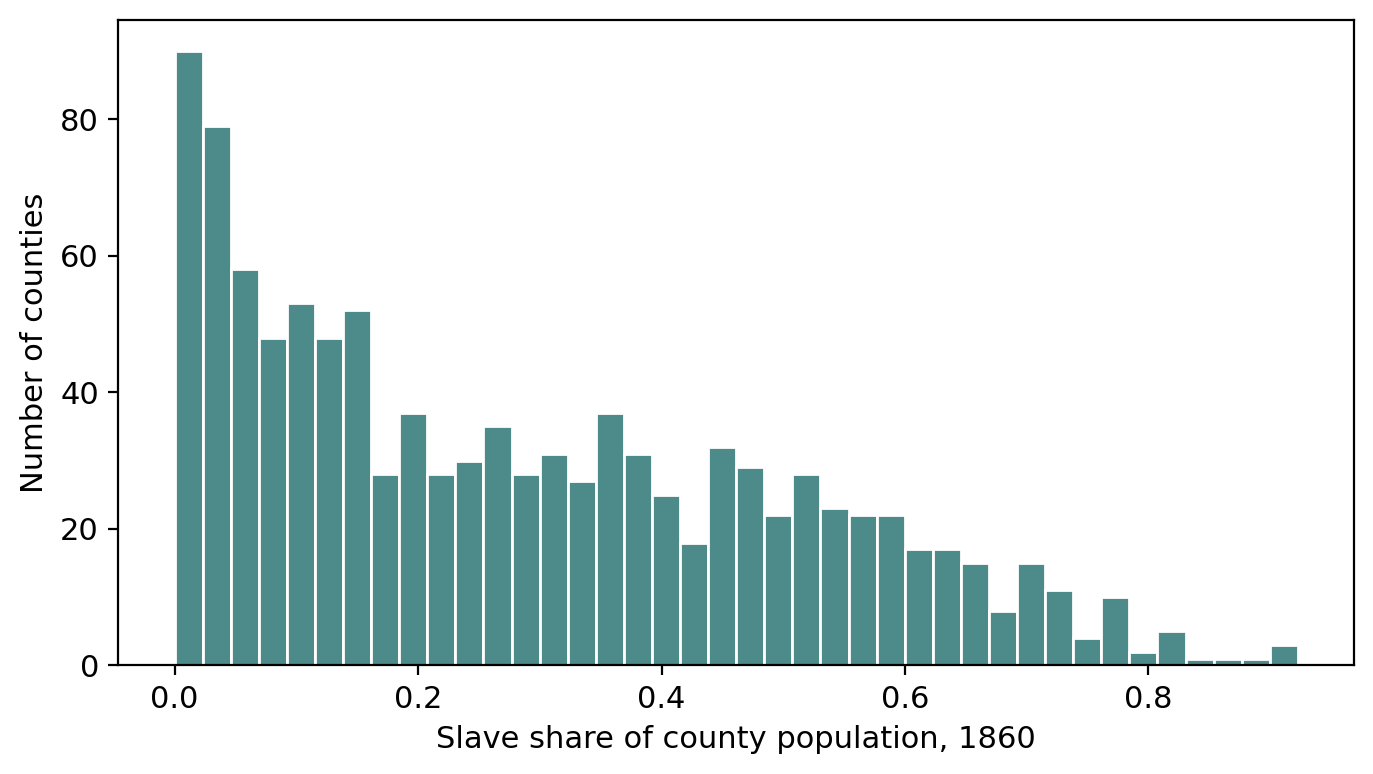
\includegraphics[width=0.7\textwidth]{output/figures/f4_hist.png}
\caption{Distribution of the 1860 enslaved share of county population across the 1,071 sample counties.}
\label{fig:hist}
\end{figure}

\newpage
\begin{thebibliography}{}

\bibitem[Acemoglu et al., 2001]{acemoglu2001}
Acemoglu, D., Johnson, S., \& Robinson, J.~A. (2001).
The colonial origins of comparative development: An empirical investigation.
\textit{American Economic Review}, 91(5), 1369--1401.

\bibitem[Acharya et al., 2016]{abs2016}
Acharya, A., Blackwell, M., \& Sen, M. (2016).
The political legacy of American slavery.
\textit{The Journal of Politics}, 78(3), 621--641.

\bibitem[Acharya et al., 2016b]{absdata}
Acharya, A., Blackwell, M., \& Sen, M. (2016b).
Replication data for: The political legacy of American slavery [dataset].
Harvard Dataverse, doi:10.7910/DVN/CAEEG7.

\bibitem[Anderson \& Rubin, 1949]{andersonrubin1949}
Anderson, T.~W., \& Rubin, H. (1949).
Estimation of the parameters of a single equation in a complete system of stochastic equations.
\textit{The Annals of Mathematical Statistics}, 20(1), 46--63.

\bibitem[Altonji et al., 2005]{altonji2005}
Altonji, J.~G., Elder, T.~E., \& Taber, C.~R. (2005).
Selection on observed and unobserved variables: Assessing the effectiveness of Catholic schools.
\textit{Journal of Political Economy}, 113(1), 151--184.

\bibitem[Becker, 1968]{becker1968}
Becker, G.~S. (1968).
Crime and punishment: An economic approach.
\textit{Journal of Political Economy}, 76(2), 169--217.

\bibitem[Bertocchi \& Dimico, 2014]{bertocchi2014}
Bertocchi, G., \& Dimico, A. (2014).
Slavery, education, and inequality.
\textit{European Economic Review}, 70, 197--209.

\bibitem[Buonanno \& Vargas, 2019]{buonanno2019}
Buonanno, P., \& Vargas, J.~F. (2019).
Inequality, crime, and the long-run legacy of slavery.
\textit{Journal of Economic Behavior \& Organization}, 159, 539--552.

\bibitem[Cameron et al., 2008]{cgm2008}
Cameron, A.~C., Gelbach, J.~B., \& Miller, D.~L. (2008).
Bootstrap-based improvements for inference with clustered errors.
\textit{The Review of Economics and Statistics}, 90(3), 414--427.

\bibitem[Conley, 1999]{conley1999}
Conley, T.~G. (1999).
GMM estimation with cross sectional dependence.
\textit{Journal of Econometrics}, 92(1), 1--45.

\bibitem[Dell, 2010]{dell2010}
Dell, M. (2010).
The persistent effects of Peru's mining mita.
\textit{Econometrica}, 78(6), 1863--1903.

\bibitem[Engerman \& Sokoloff, 2002]{engerman2002}
Engerman, S.~L., \& Sokoloff, K.~L. (2002).
Factor endowments, inequality, and paths of development among New World economies.
NBER Working Paper No.~9259.

\bibitem[Fajnzylber et al., 2002]{fajnzylber2002}
Fajnzylber, P., Lederman, D., \& Loayza, N. (2002).
Inequality and violent crime.
\textit{The Journal of Law and Economics}, 45(1), 1--39.

\bibitem[Foner, 1988]{foner1988}
Foner, E. (1988).
\textit{Reconstruction: America's Unfinished Revolution, 1863--1877}.
New York: Harper \& Row.

\bibitem[Glaeser et al., 1996]{glaeser1996}
Glaeser, E.~L., Sacerdote, B., \& Scheinkman, J.~A. (1996).
Crime and social interactions.
\textit{The Quarterly Journal of Economics}, 111(2), 507--548.

\bibitem[Gouda \& Rigterink, 2025]{gouda2025}
Gouda, M., \& Rigterink, A.~S. (2025).
Historical slavery predicts contemporary violent crime: Inequality and political attitudes as mediators.
\textit{Social Science Quarterly}, 106, e70078.

\bibitem[Kelly, 2000]{kelly2000}
Kelly, M. (2000).
Inequality and crime.
\textit{The Review of Economics and Statistics}, 82(4), 530--539.

\bibitem[Manson et al., 2023]{nhgis}
Manson, S., Schroeder, J., Van Riper, D., Knowles, K., Kugler, T., Roberts, F., \& Ruggles, S. (2023).
IPUMS National Historical Geographic Information System: Version 18.0 [dataset].
Minneapolis, MN: IPUMS.

\bibitem[Nunn, 2008a]{nunn2008qje}
Nunn, N. (2008a).
The long-term effects of Africa's slave trades.
\textit{The Quarterly Journal of Economics}, 123(1), 139--176.

\bibitem[Nunn, 2008b]{nunn2008americas}
Nunn, N. (2008b).
Slavery, inequality, and economic development in the Americas: An examination of the Engerman--Sokoloff hypothesis.
In E.~Helpman (Ed.), \textit{Institutions and Economic Performance} (pp.~148--180). Cambridge, MA: Harvard University Press.

\bibitem[O'Connell, 2012]{oconnell2012}
O'Connell, H.~A. (2012).
The impact of slavery on racial inequality in poverty in the contemporary U.S. South.
\textit{Social Forces}, 90(3), 713--734.

\bibitem[Pazzona, 2024]{pazzona2024}
Pazzona, M. (2024).
Revisiting the income inequality--crime puzzle.
\textit{World Development}, 176, 106520.

\bibitem[Sacerdote, 2005]{sacerdote2005}
Sacerdote, B. (2005).
Slavery and the intergenerational transmission of human capital.
\textit{The Review of Economics and Statistics}, 87(2), 217--234.

\bibitem[Santos Silva \& Tenreyro, 2006]{santossilva2006}
Santos Silva, J.~M.~C., \& Tenreyro, S. (2006).
The log of gravity.
\textit{The Review of Economics and Statistics}, 88(4), 641--658.

\bibitem[Staiger \& Stock, 1997]{staigerstock1997}
Staiger, D., \& Stock, J.~H. (1997).
Instrumental variables regression with weak instruments.
\textit{Econometrica}, 65(3), 557--586.

\bibitem[Tolnay \& Beck, 1995]{tolnay1995}
Tolnay, S.~E., \& Beck, E.~M. (1995).
\textit{A Festival of Violence: An Analysis of Southern Lynchings, 1882--1930}.
Urbana: University of Illinois Press.

\bibitem[U.S. DOJ/FBI, var.]{ucr2010}
U.S. Department of Justice, Federal Bureau of Investigation.
\textit{Uniform Crime Reporting Program Data: County-Level Detailed Arrest and Offense Data} [United States], 1990 (ICPSR 9785), 2000 (ICPSR 3451), 2010 (ICPSR 33523), 2016 (ICPSR 37059).
Ann Arbor, MI: Inter-university Consortium for Political and Social Research.

\end{thebibliography}

\end{document}
